
\documentclass[compress]{beamer}

\usetheme{metropolis}


%\usetheme[compress]{Singapore}

\usepackage{amssymb}
\usepackage{amsmath}
\usepackage{graphicx}
\graphicspath{ {Graficos/} }
\usepackage{subfigure}
\usepackage{booktabs} % Allows the use of \toprule, \midrule and \bottomrule in tables
\usepackage{caption}
\newcommand*{\boxedcolor}{red}

\makeatletter
\setbeamertemplate{headline}{%
  \begin{beamercolorbox}[colsep=0pt]{upper separation line head}
  \end{beamercolorbox}
  \begin{beamercolorbox}{section in head/foot}
    \vskip2pt\insertnavigation{\paperwidth}\vskip2pt
  \end{beamercolorbox}%
  \begin{beamercolorbox}[colsep=0pt]{lower separation line head}
  \end{beamercolorbox}
}
\makeatother

\setbeamercolor{section in head/foot}{fg=normal text.bg, bg=structure.fg}



%%%%%%%%%%%% TITULO %%%%%%%%%%%%

\title[Defensa de Tesis]{Análisis empírico del comercio internacional a partir de la segunda mitad del siglo XX.}

\subtitle{Propuestas metodológicas basadas en teoría de grafos y modelos generativos
	bayesianos}


\author{Diego Kozlowski}
\institute[Universidad de Buenos Aires]
{
	Universidad de Buenos Aires\\ 
	
	\textit{Master en Data Mining \& Knowledge Discovery} \\
	\medskip
	\textit{Supervisor: Viktoriya Semeshenko}
}
\date{}



\usepackage{enumitem}

\usepackage{fdsymbol}
\usepackage{fontawesome}


\begin{document}

\begin{frame}

\titlepage 

\end{frame}


%		\section{Topic}

\begin{frame}

\section{Introducción}


\frametitle{Tema}

\begin{itemize}
	
	\item[\faRebel] Los datos de comercio internacional son flujos de importaciones y exportaciones entre países, para un período de tiempo 
	\item[\faRebel] Es un problema de alta dimensionalidad: país-año-producto-tipo de flujo
	\item[\faRebel] el \textbf{objetivo} de esta tesis es construir un sistema de representación de la información que comprenda las múltiples dimensiones.
	\item[\faRebel] Esto es realizado utilizando técnicas de Análisis exploratorio de datos, Redes complejas y modelos generativos bayesianos. 
\end{itemize}

\end{frame}


\begin{frame}
\frametitle{Fuentes de información}

\begin{itemize}
	
	\item[\faRebel] Comercio agregado por país y año. 1948-2016\footnote{Gleditsch \url{http://ksgleditsch.com/exptradegdp.html}}  
	\item[\faRebel] Comercio desagregado a nivel producto, año y país. 1997-2016\footnote{Organización mundial del comercio \url{https://comtrade.un.org/}}
	\item[\faRebel] Comercio desagregado a nivel producto, año y país. 1962-2016\footnote{The Atlas of Economic Complexity \url{http://www.atlas.cid.harvard.edu.}}	
\end{itemize}

\end{frame}


\section{Metodología}

\subsection{Comercio Agregado}
\begin{frame}
\begin{columns}[c] 

\column{.45\textwidth} % Right column and width
\begin{figure}
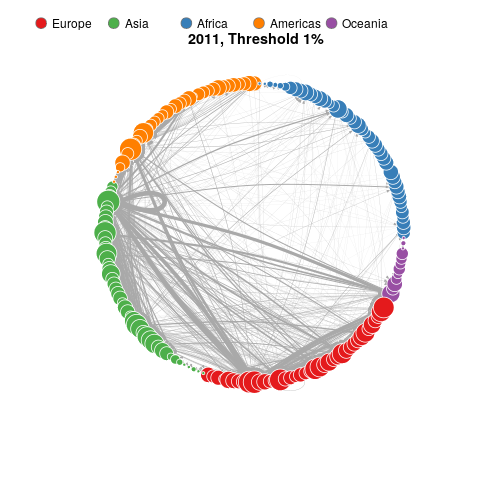
\includegraphics[width=1.4\linewidth]{grafo_Circ_2011_1_pcnt}
\end{figure}

\column{.5\textwidth} % Left column and width
\small

\begin{itemize}
	
	\item[\faRebel] Grafo dirigido no ponderado de \textit{comercio bilateral por año y tipo} 
	\item[\faRebel] Análisis de puntos de corte y medidas de centralidad
	\item[\faRebel] El rol de los países en el comercio mundial basado en su posición en el grafo	
\end{itemize}


\end{columns}
\end{frame}

		\begin{frame}
\frametitle{Comercio Bilateral}

\begin{columns}[t]
	\column{.5\textwidth}
	
	$$
	a_{ij} = 
	\begin{cases} 
	1 & si \ \frac{x_{ij}}{x_{i\cdot}}\geq u \\
	0 & sino 
	\end{cases}
	$$
	$x_{ij}$: Comercio total entre los países i-j \par
	$x_{i\cdot}$: Comercio total del país i
	
	\column{.5\textwidth}
	
	\begin{itemize}[label=\faRebel]
		\item Dos países están conectados si existe \textit{suficiente} comercio entre ellos.
		\item Puede ser tanto expo como impo.
		\item El grafo es dirigido, por lo que $a_{ij} \neq a_{ji}$.
	\end{itemize}
	
\end{columns}

\end{frame}



\begin{frame}
\frametitle{Productores \& Consumidores}	
\begin{columns}
\column{.5\textwidth}
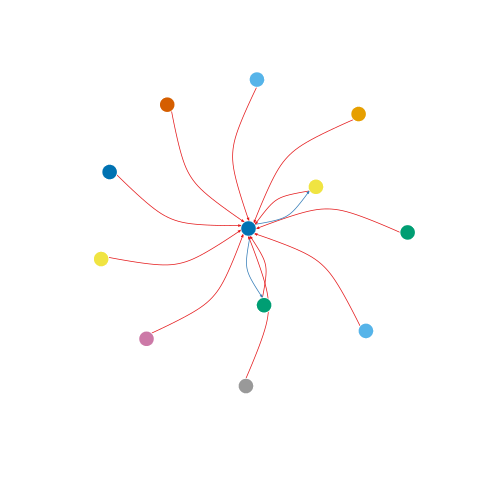
\includegraphics[width=\linewidth]{toy_graph1}

\column{.65\textwidth}
\begin{itemize}[label=\faRebel]
	\item Desde el punto de vista de un país, no puede haber muchos países relevantes, $\therefore$ no hay muchas \textbf{aristas de salida}
	\item Pero puede ser relevante desde el punto de vista de muchos otros países.
	$\therefore$ puede recibir muchas \textbf{aristas de entrada}
	\item Con datos de \textbf{expo}, un nodo central es \textbf{importante como consumidor}
	\item Con datos de \textbf{impo}, un nodo central es \textbf{importante como productor}
\end{itemize}	
\end{columns}	
\end{frame}



\subsection{disaggregated trade}
\begin{frame}

\begin{columns}[c] 

\column{.45\textwidth} % Right column and width
$$
RCA(c,i)= \frac{\displaystyle \frac{x(c,i)}{\displaystyle \sum_{i}x(c,i)}}{\frac{\displaystyle\sum_{c}x(c,i)}{\displaystyle \sum_{c,i}x(c,i)}}
$$	
\column{.5\textwidth} % Left column and width
\small

\begin{itemize}
	
	\item[\faRebel] Composición de las canastas de exportación-importación en países Latinoamericanos 
	\item[\faRebel] Grafo bipartito entre países y productos
	\item[\faRebel] Relative Comparative Advantages basado en 	(\textit{Hidalgo and Hausmann, 2009})
\end{itemize}

\end{columns}



\end{frame}

\subsection{Latent Dirichlet Allocation Model}
\begin{frame}

\frametitle{Modelo de Latent Dirichlet Allocation}

\begin{columns}[c] 

\column{.45\textwidth} % Right column and width
\begin{figure}
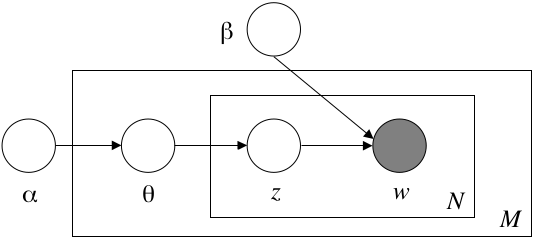
\includegraphics[width=\linewidth]{grafo}

\medskip
\tiny
$\beta \sim Dir_v(\eta)$  Distribución de productos en los componentes latentes\\
$\theta_d \sim Dir_K(\alpha)$ : Distribución de los componentes latentes por país\\
$z_{dn} \sim Mult(\theta_d)$ : Componente latente \\
$w_{dn} \sim Mult(\beta_{zn})$: u\$s comerciado

\end{figure}

\column{.5\textwidth} % Left column and width
\small

\begin{itemize}
	
	\item[\faRebel] Basado en Topic Modeling  (\textit{David M. Blei Andrew Y. Ng, 2003}) realizamos inferencia sobre los \textit{componentes latentes} en el comercio internacional utilizando un modelo de inferencia bayesiana
	\item[\faRebel] Cómo resultado, obtenemos la distribución de los productos sobre los componentes latentes, y la distribución de los componentes sobre los países
\end{itemize}

\end{columns}
\end{frame}

\section{Resultados}


\begin{frame}

\scriptsize{
\textbf{Determinación del Punto de corte}. En 1\% se obtiene una red densamente conectada con máximo clustering (deseable si el objetivo es poder agrupar a países según sus características en el grafo)}

	\begin{figure}
		\centering
		\subfigure[1\%]{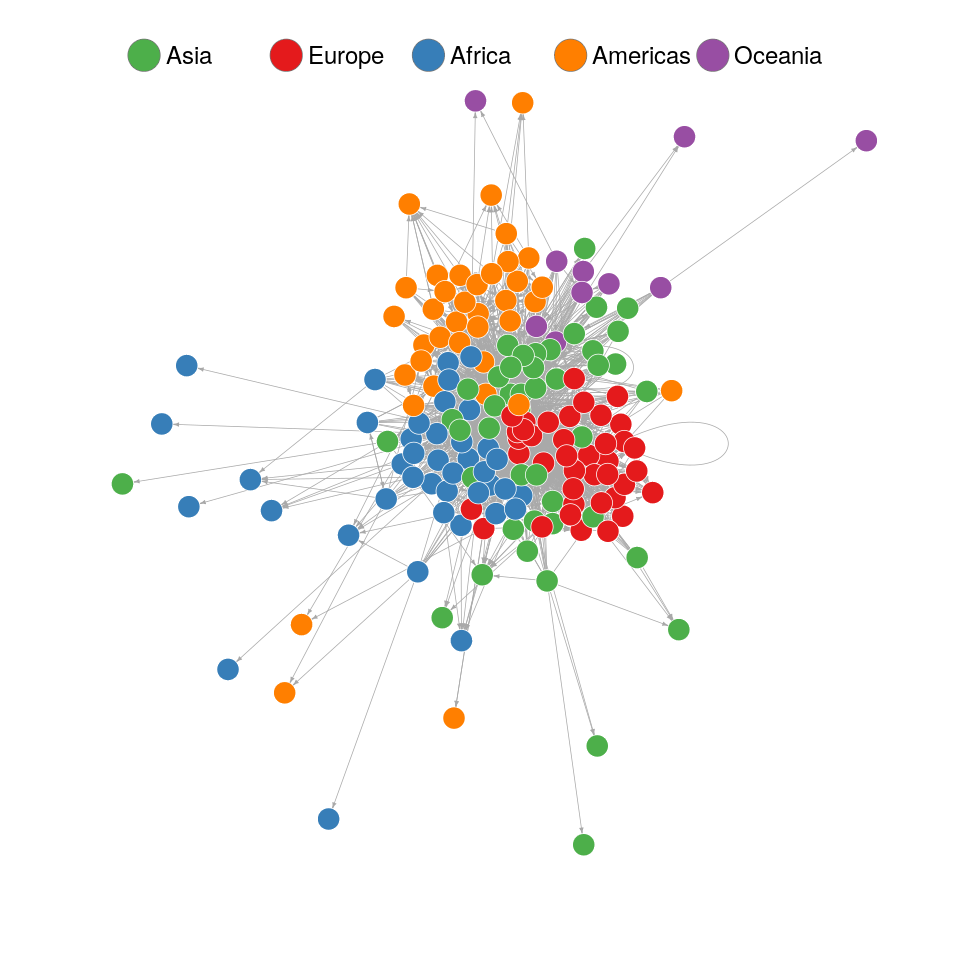
\includegraphics[width=0.2\linewidth]{grafo_2016_1_pcnt}}
		\subfigure[5\%]{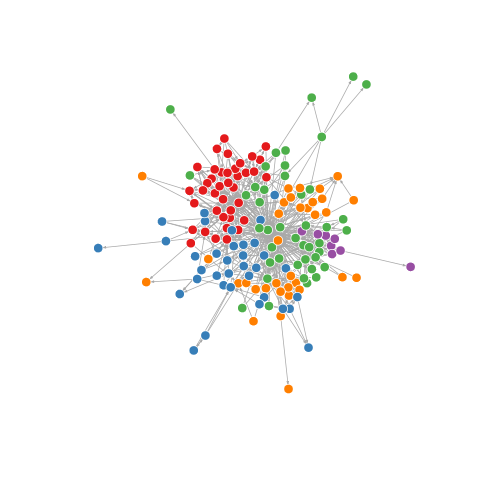
\includegraphics[width=0.2\linewidth]{grafo_2016_5_pcnt}}
		\subfigure[10\%]{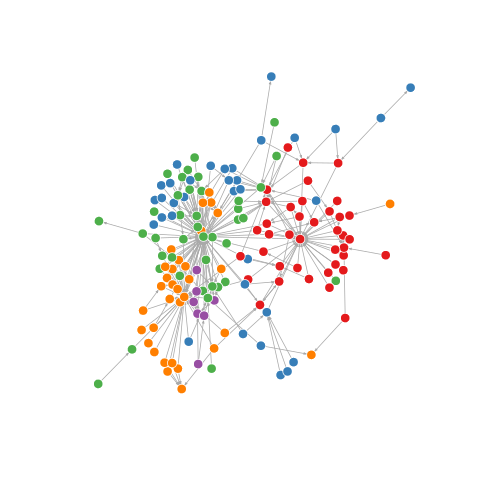
\includegraphics[width=0.2\linewidth]{grafo_2016_10_pcnt}}
		\subfigure[15\%]{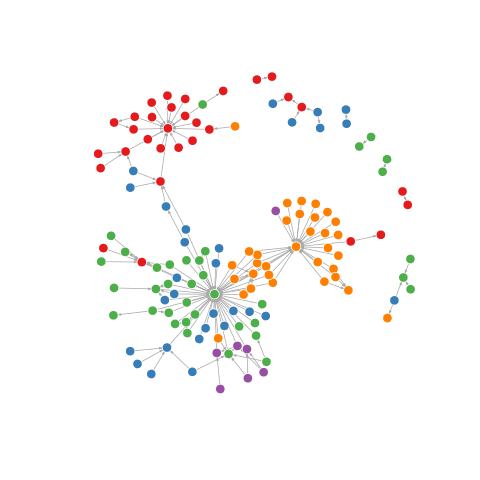
\includegraphics[width=0.2\linewidth]{grafo_2016_15_pcnt}}
		\subfigure[20\%]{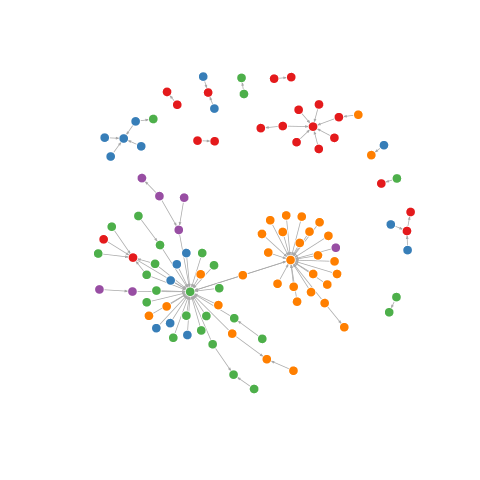
\includegraphics[width=0.2\linewidth]{grafo_2016_20_pcnt}}
		\subfigure[25\%]{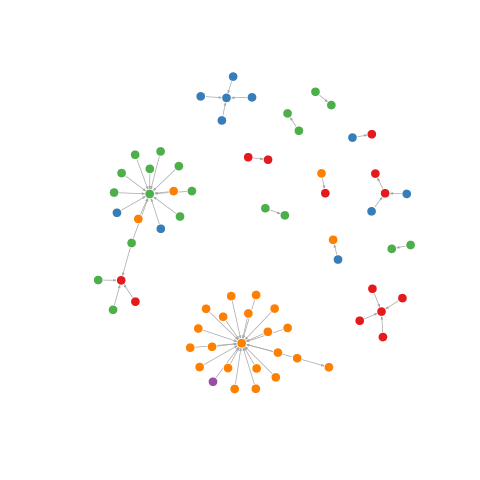
\includegraphics[width=0.2\linewidth]{grafo_2016_25_pcnt}}
		\subfigure[Clustering]{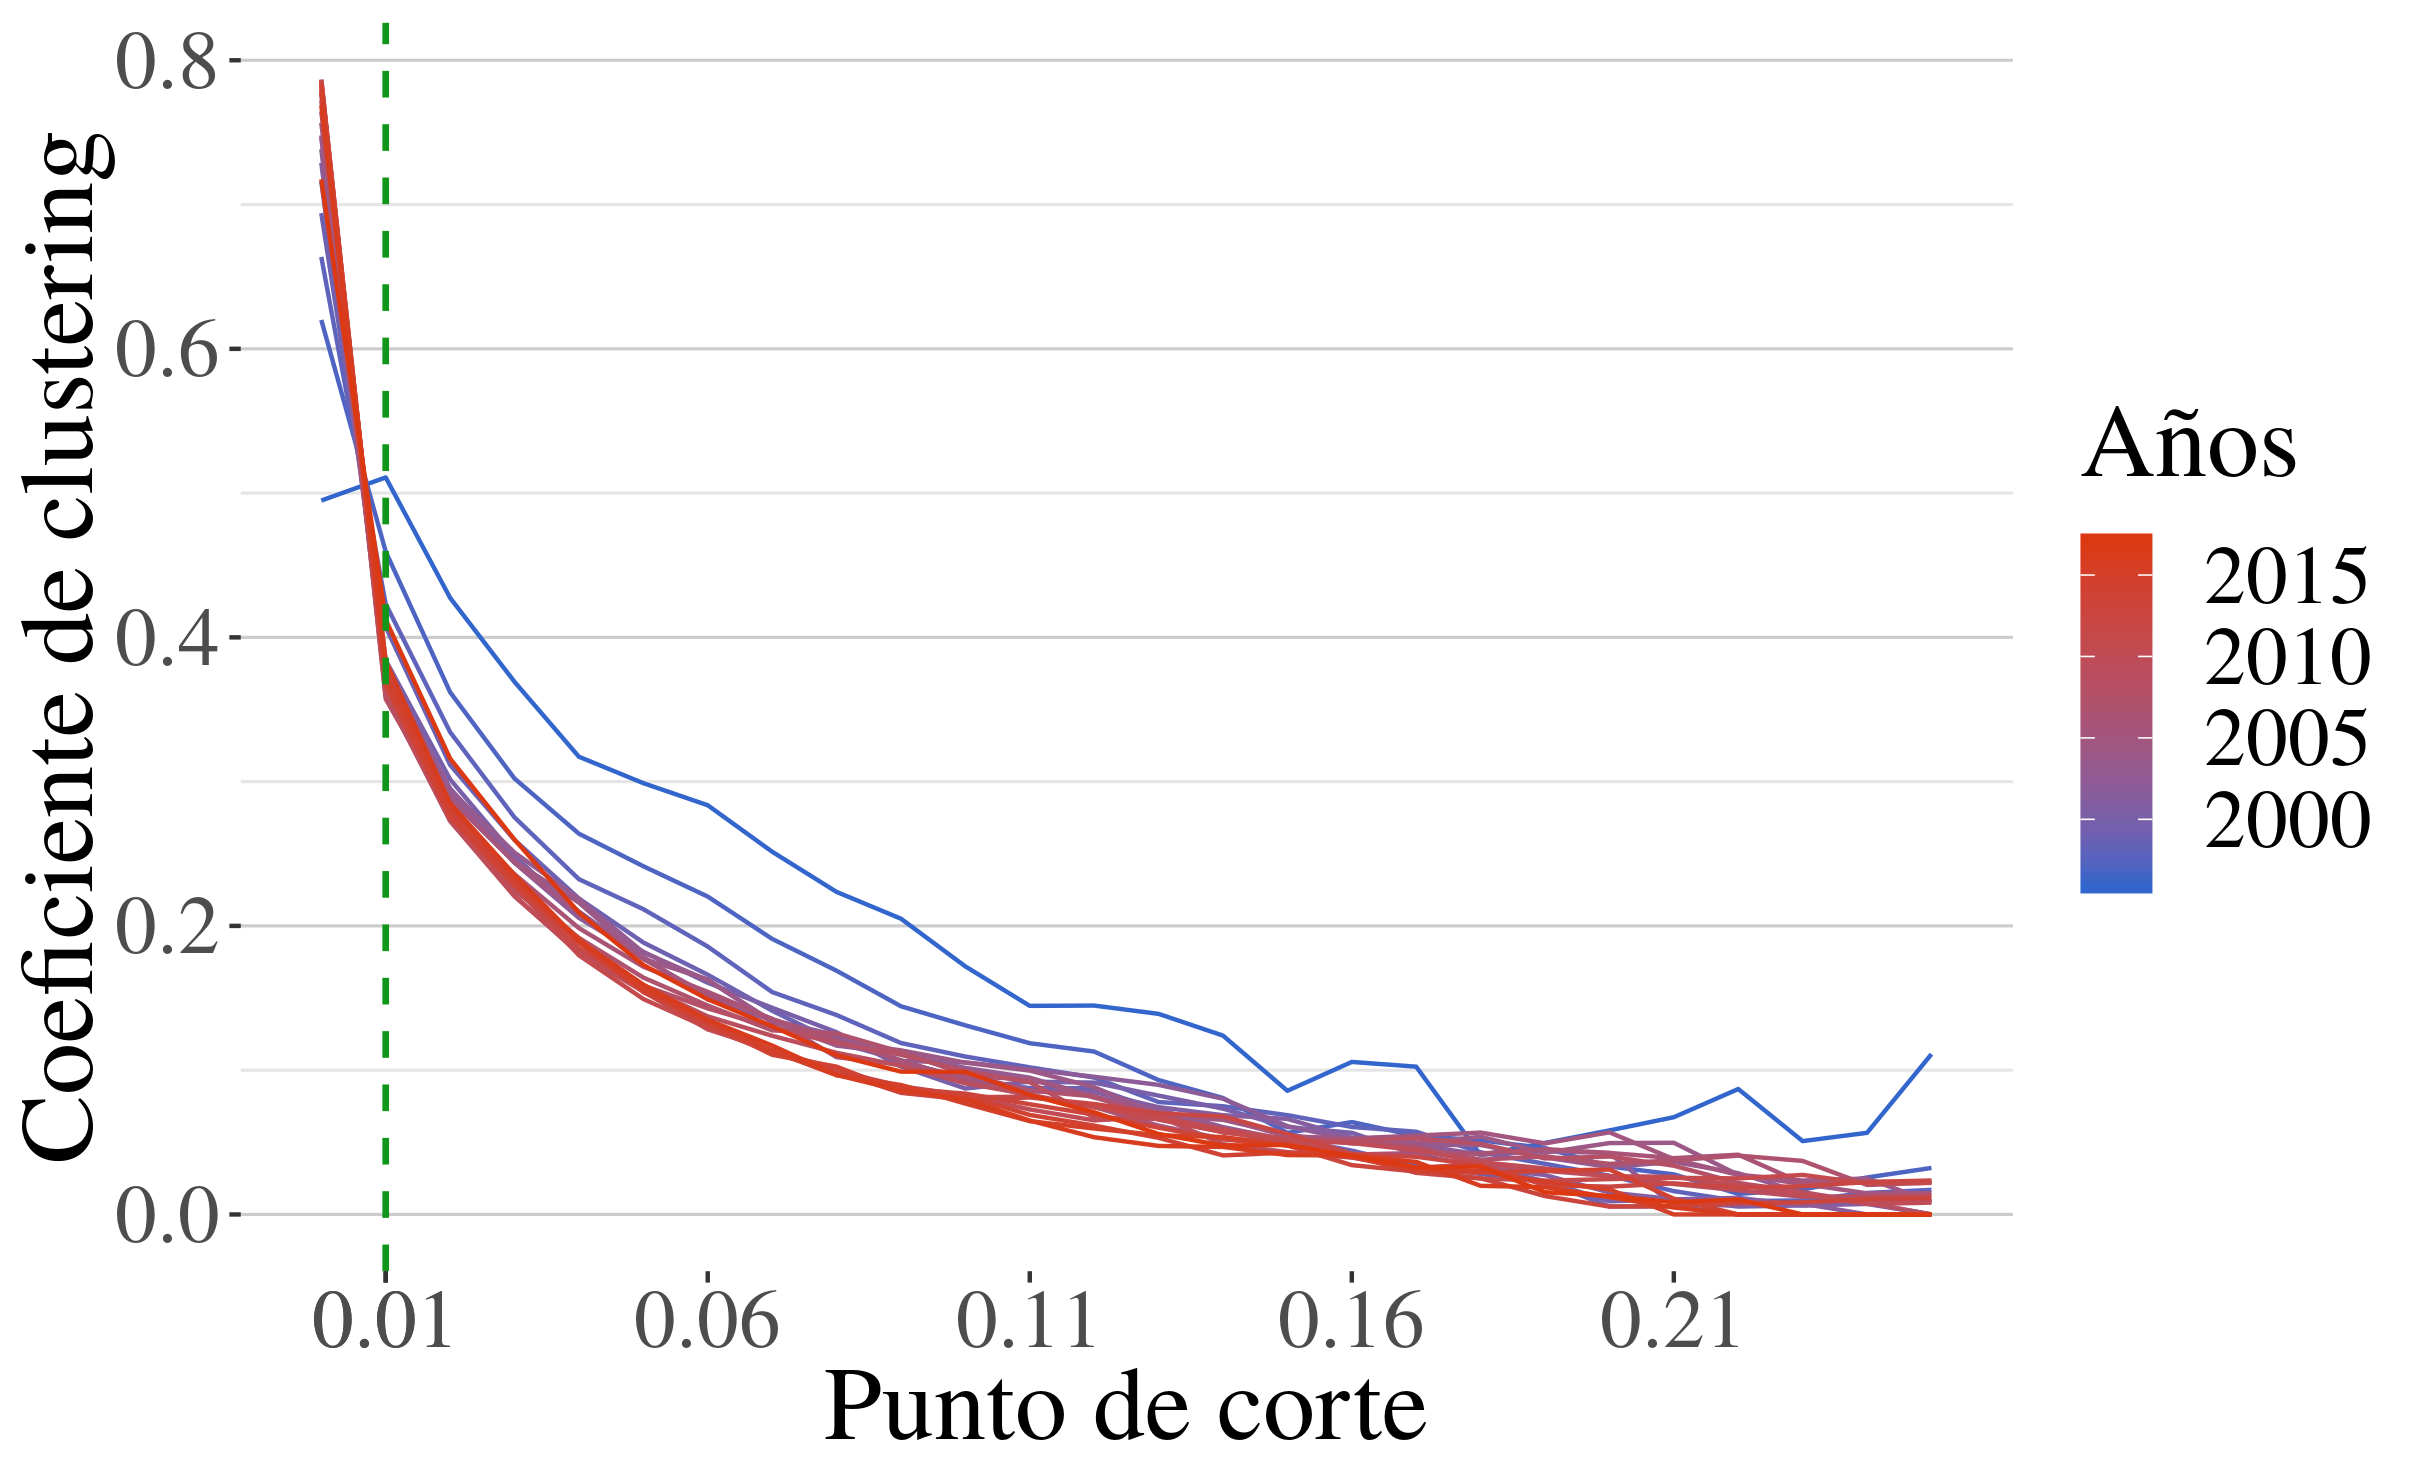
\includegraphics[width=0.4\linewidth]{threshold_x_clustering_x_yr}}
		\caption{Grafos. 2016, según punto de corte}
		\label{fig:grafo_2016}
	\end{figure}
	
\end{frame}




\subsection{Exports and Imports correlation}
\begin{frame}

%The relation of the centrality measures between exports and imports networks for a given year shows the relative position in word trade of the countries/continents	

\frametitle{Correlación Expo-Impo.}

punto de corte: 1\%.
Coeficiente de Pearson= 0.96

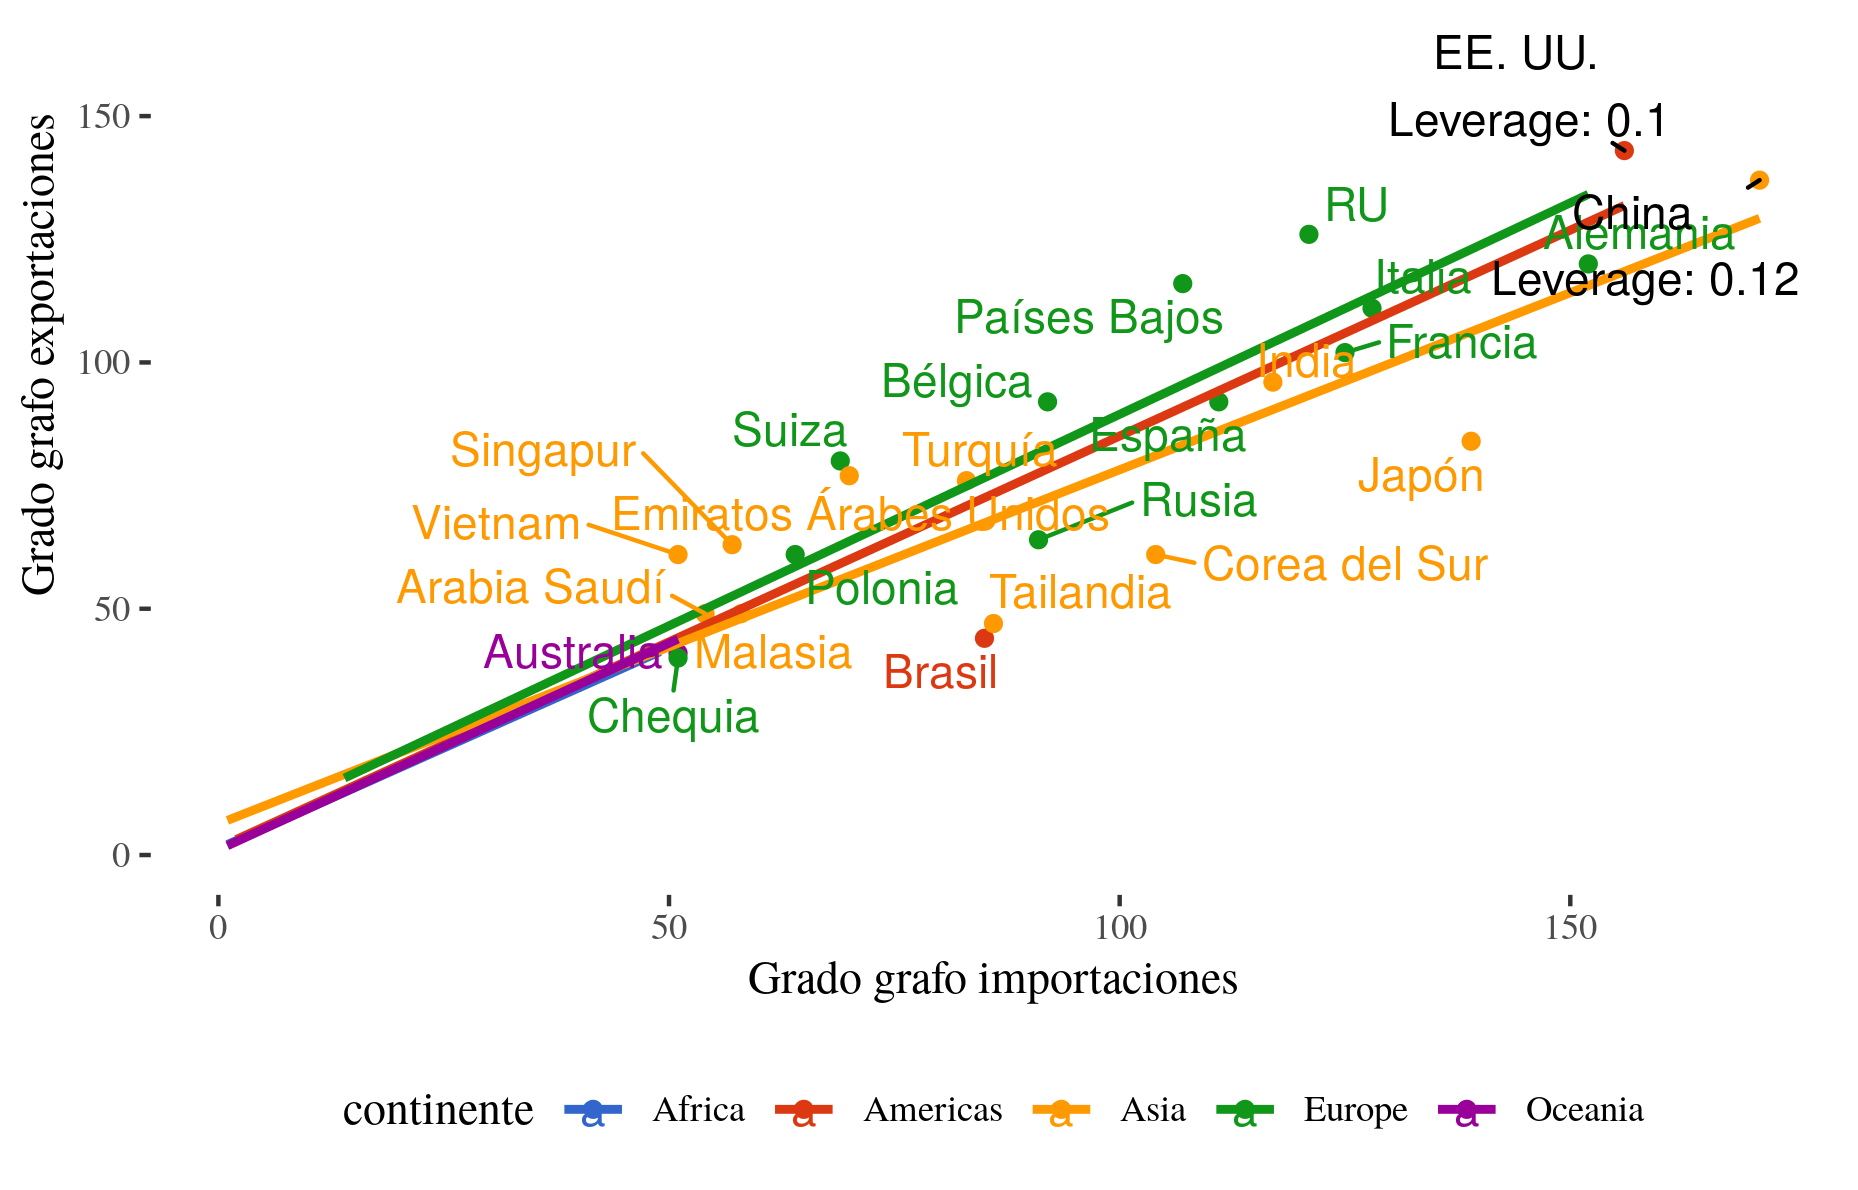
\includegraphics[width=\linewidth]{Graficos/corr_grados_2016_1_pcnt}

\end{frame}

\begin{frame}

\begin{itemize}
	\item[\faRebel] Por la forma de construcción, una mayor centralidad en el grafo de las importaciones denota una importancia del país como productor para el mercado mundial, mientras que una mayor centralidad con el grafo de exportaciones denota importancia como consumidor.
	\item[\faRebel] Podemos ver que hay una correlación alta entre ambos grafos, pero también que países como Bélgica o Suiza son más importantes como consumidores de mercancías.
	\item[\faRebel] Corea del Sur, Japón y Brasil, por su parte, son más importantes como productores de mercancías. 
\end{itemize}
\end{frame}


\begin{frame}
\frametitle{Correlación Expo-Impo.}

punto de corte: 10\%.
Coeficiente de Pearson= 0.77

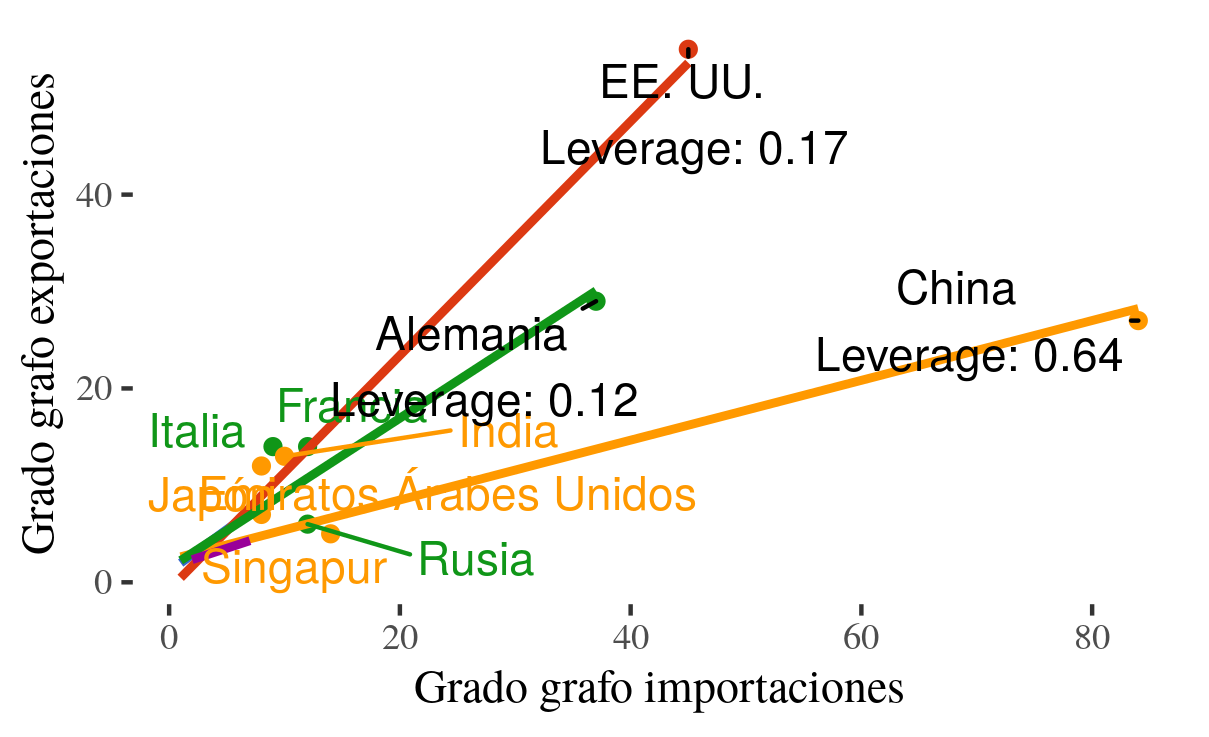
\includegraphics[width=\linewidth]{Graficos/corr_grados_2016_10_pcnt}

\end{frame}

\begin{frame}

\begin{itemize}
	\item[\faRebel] Un punto de corte más alto implica relaciones de mayor dependencia.
	\item[\faRebel] En este tipo de relaciones destacan menos países, con mayor leverage 
\end{itemize}
\end{frame}


\begin{frame}
\frametitle{Correlación Expo-Impo.}

punto de corte: 20\%.
Coeficiente de Pearson= 0.81

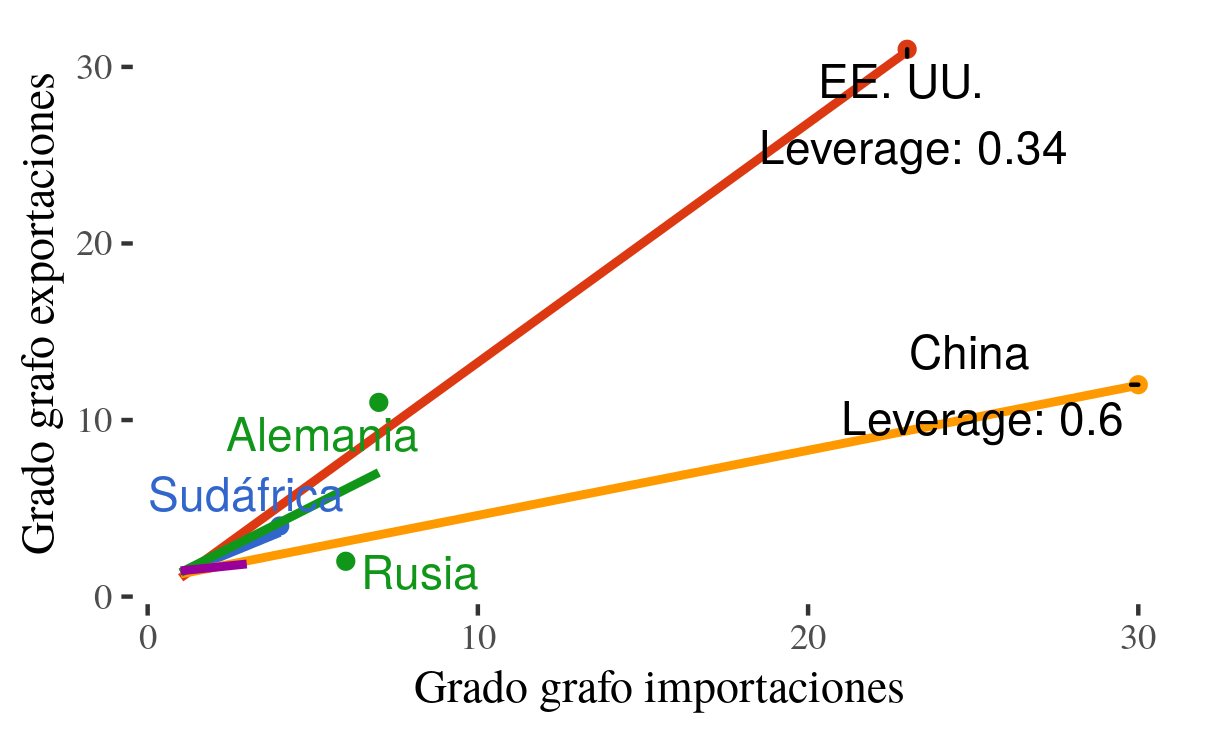
\includegraphics[width=\linewidth]{Graficos/corr_grados_2016_20_pcnt}

\end{frame}

\begin{frame}

\begin{itemize}
	\item[\faRebel] En el extremo, en relaciones de \textit{alta dependencia} destacan sobretodo Estados Unidos como consumidor, y China como productor.
	\item[\faRebel] Alemania, Sudáfrica y Rusia también destacan por tener relaciones de alta dependencia. 
\end{itemize}
\end{frame}


\subsection{Aggregated Trade}
\begin{frame}	
\small{Evolución de la distribución de la centralidad de grado en el tiempo. China y EEUU destacado}

\begin{columns}[c] 


\column{.45\textwidth} % Right column and width
\begin{figure}
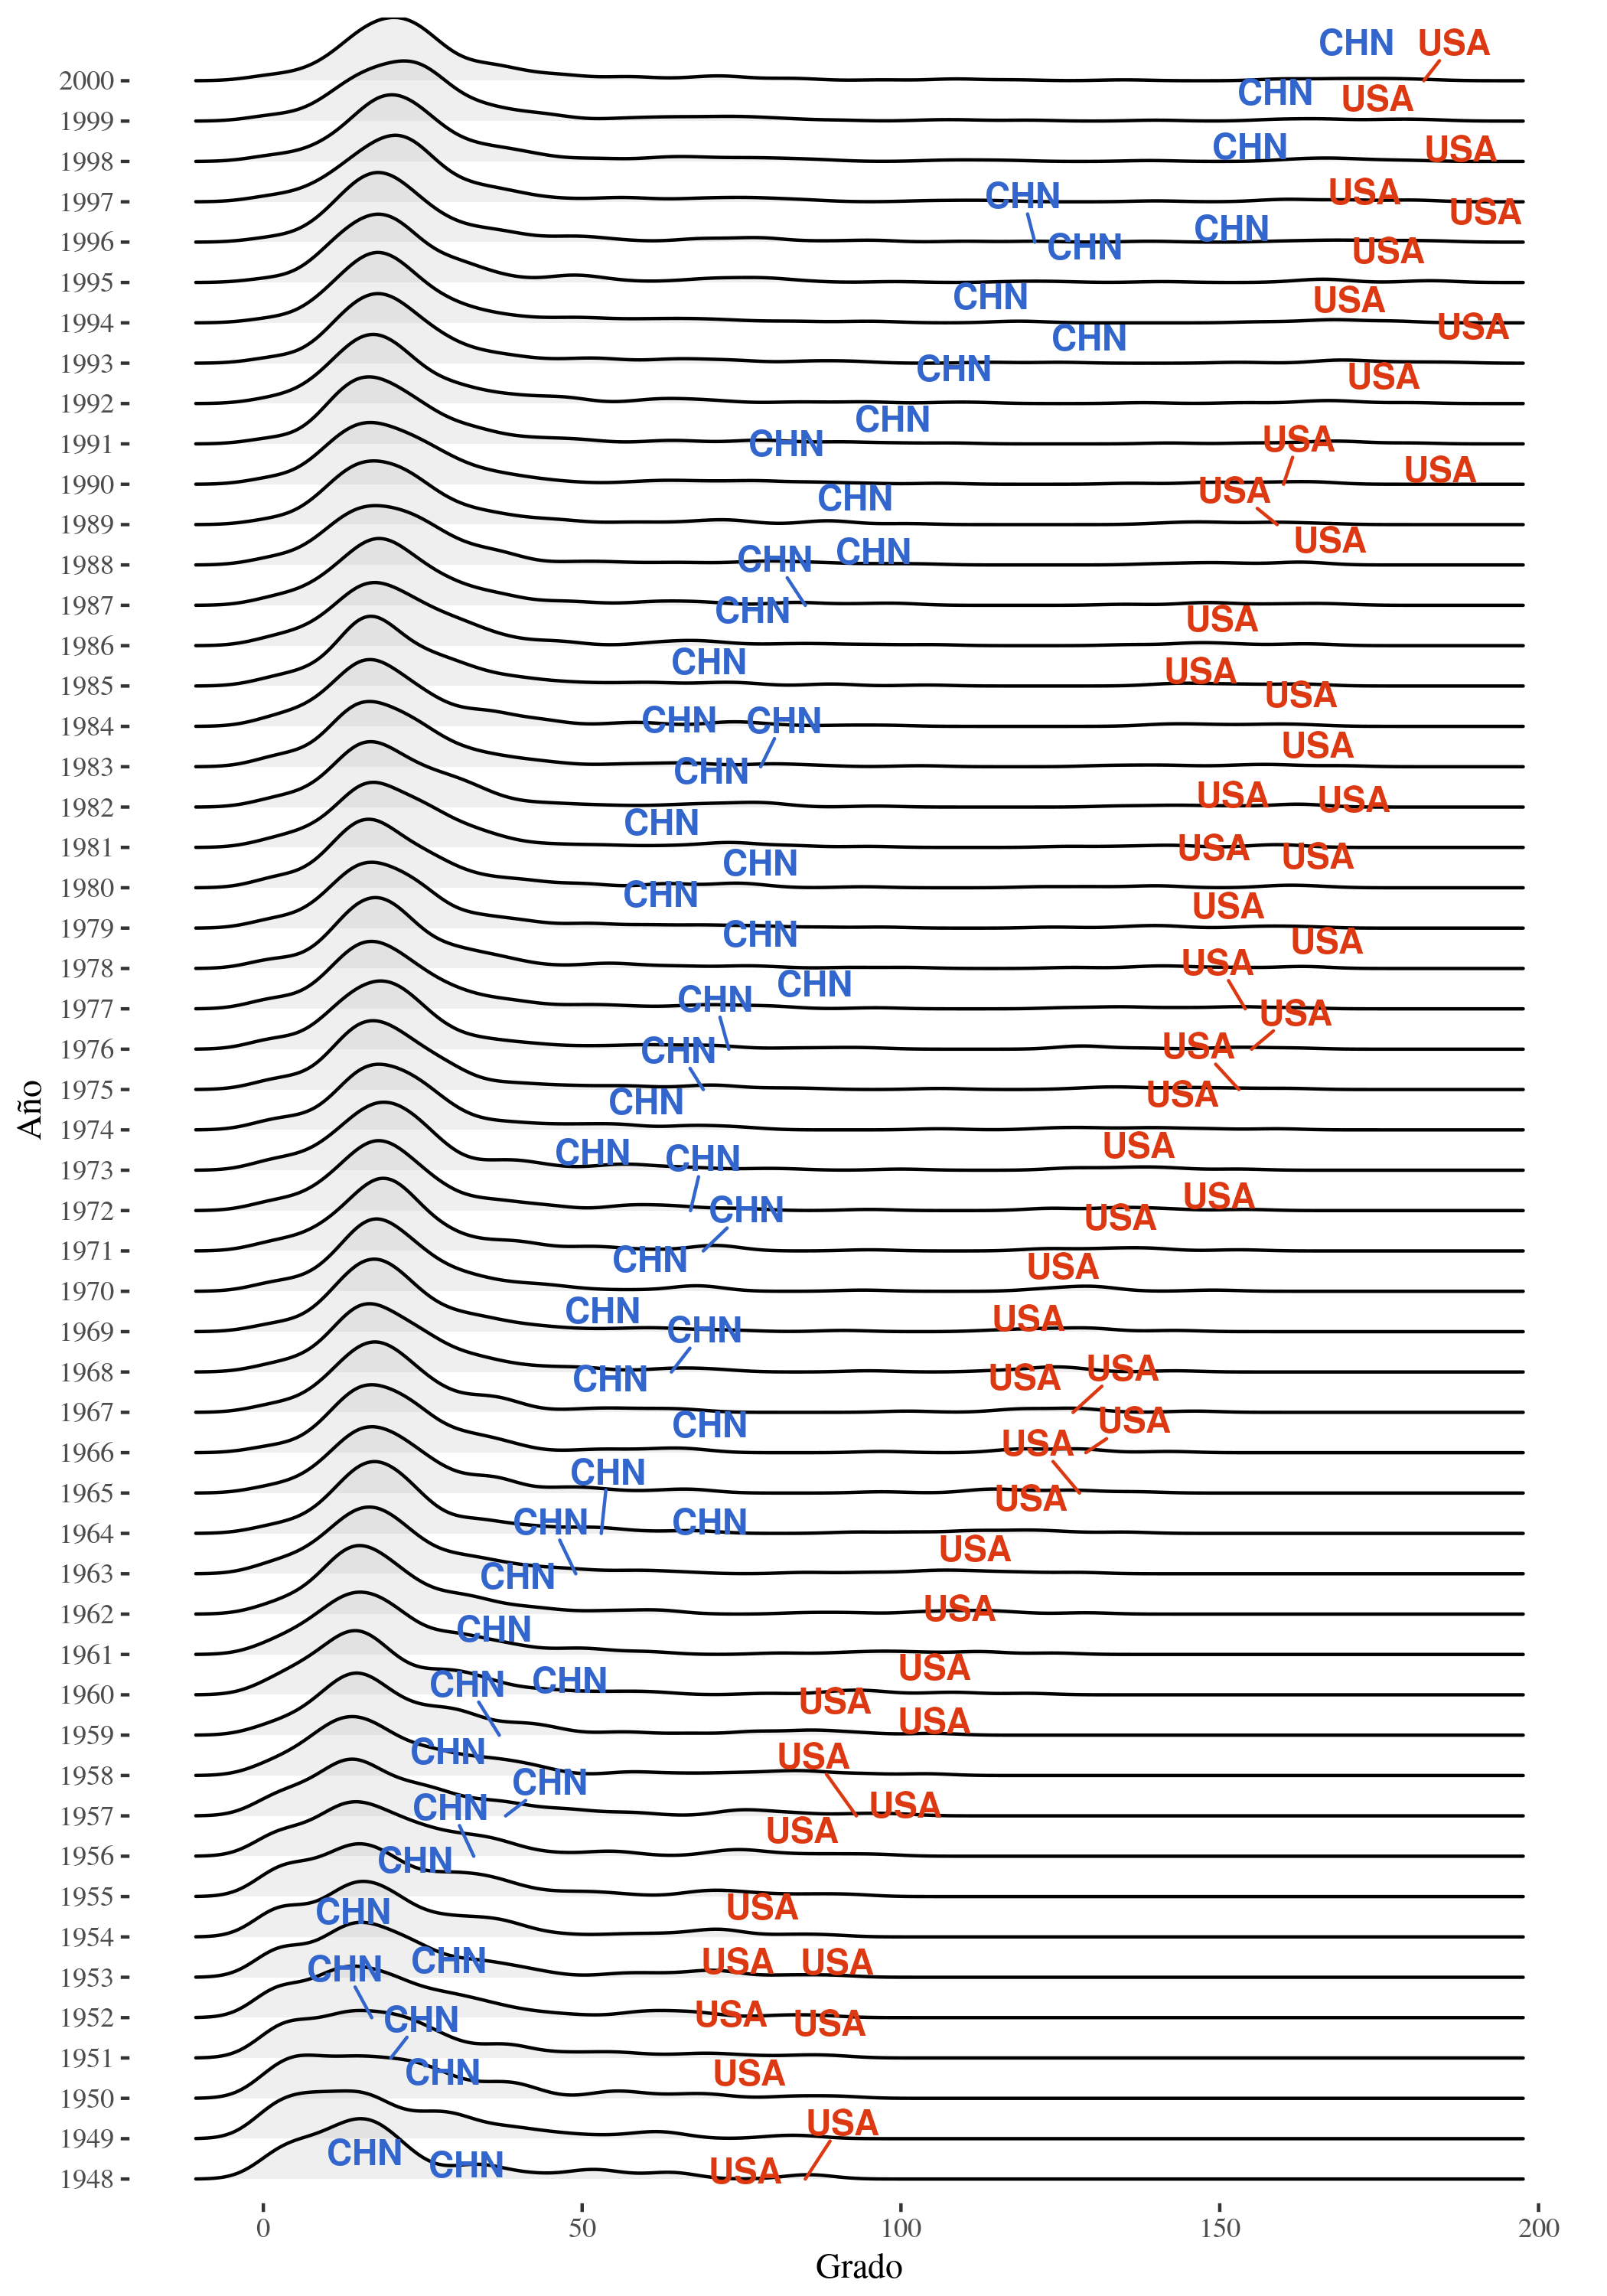
\includegraphics[scale=0.25]{1950_2000_impo_densidad_USA_CHN_grado}
\end{figure}

\column{.5\textwidth} % Left column and width

\begin{flushleft}
\begin{figure}
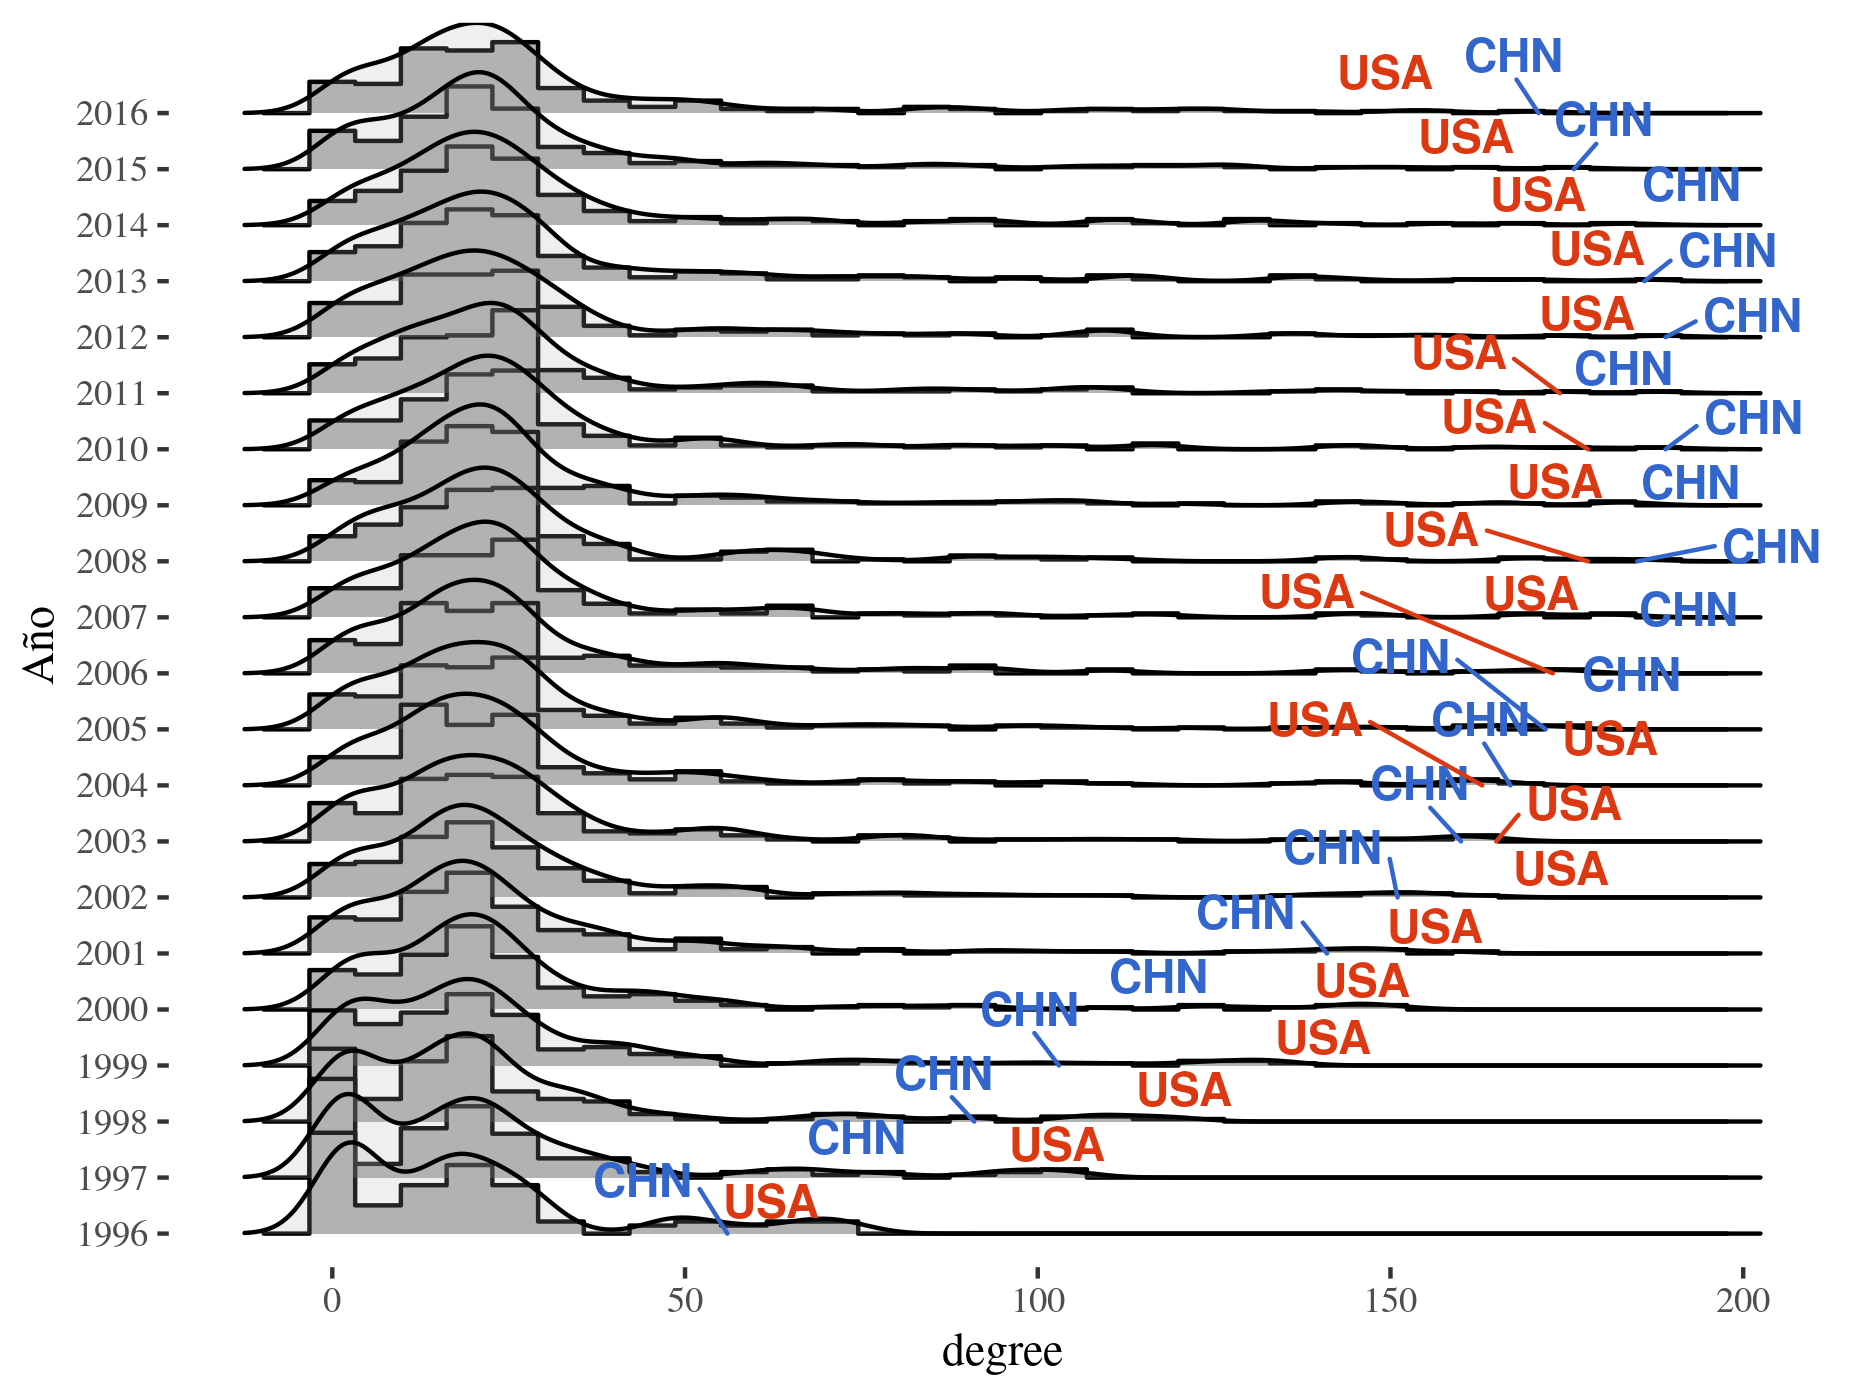
\includegraphics[scale=0.35]{impo_densidad_USAvsCHN_grado_x_yr}
\end{figure}
\end{flushleft}

\end{columns}
\small{Más resultados en: \textbf{\url{https://diegokoz.shinyapps.io/Distribucion_nodos_wrdtrade/}}}
\end{frame}

\begin{frame}
\begin{figure}
	
	\centering
	\subfigure{\label{fig:metricas_LP-a}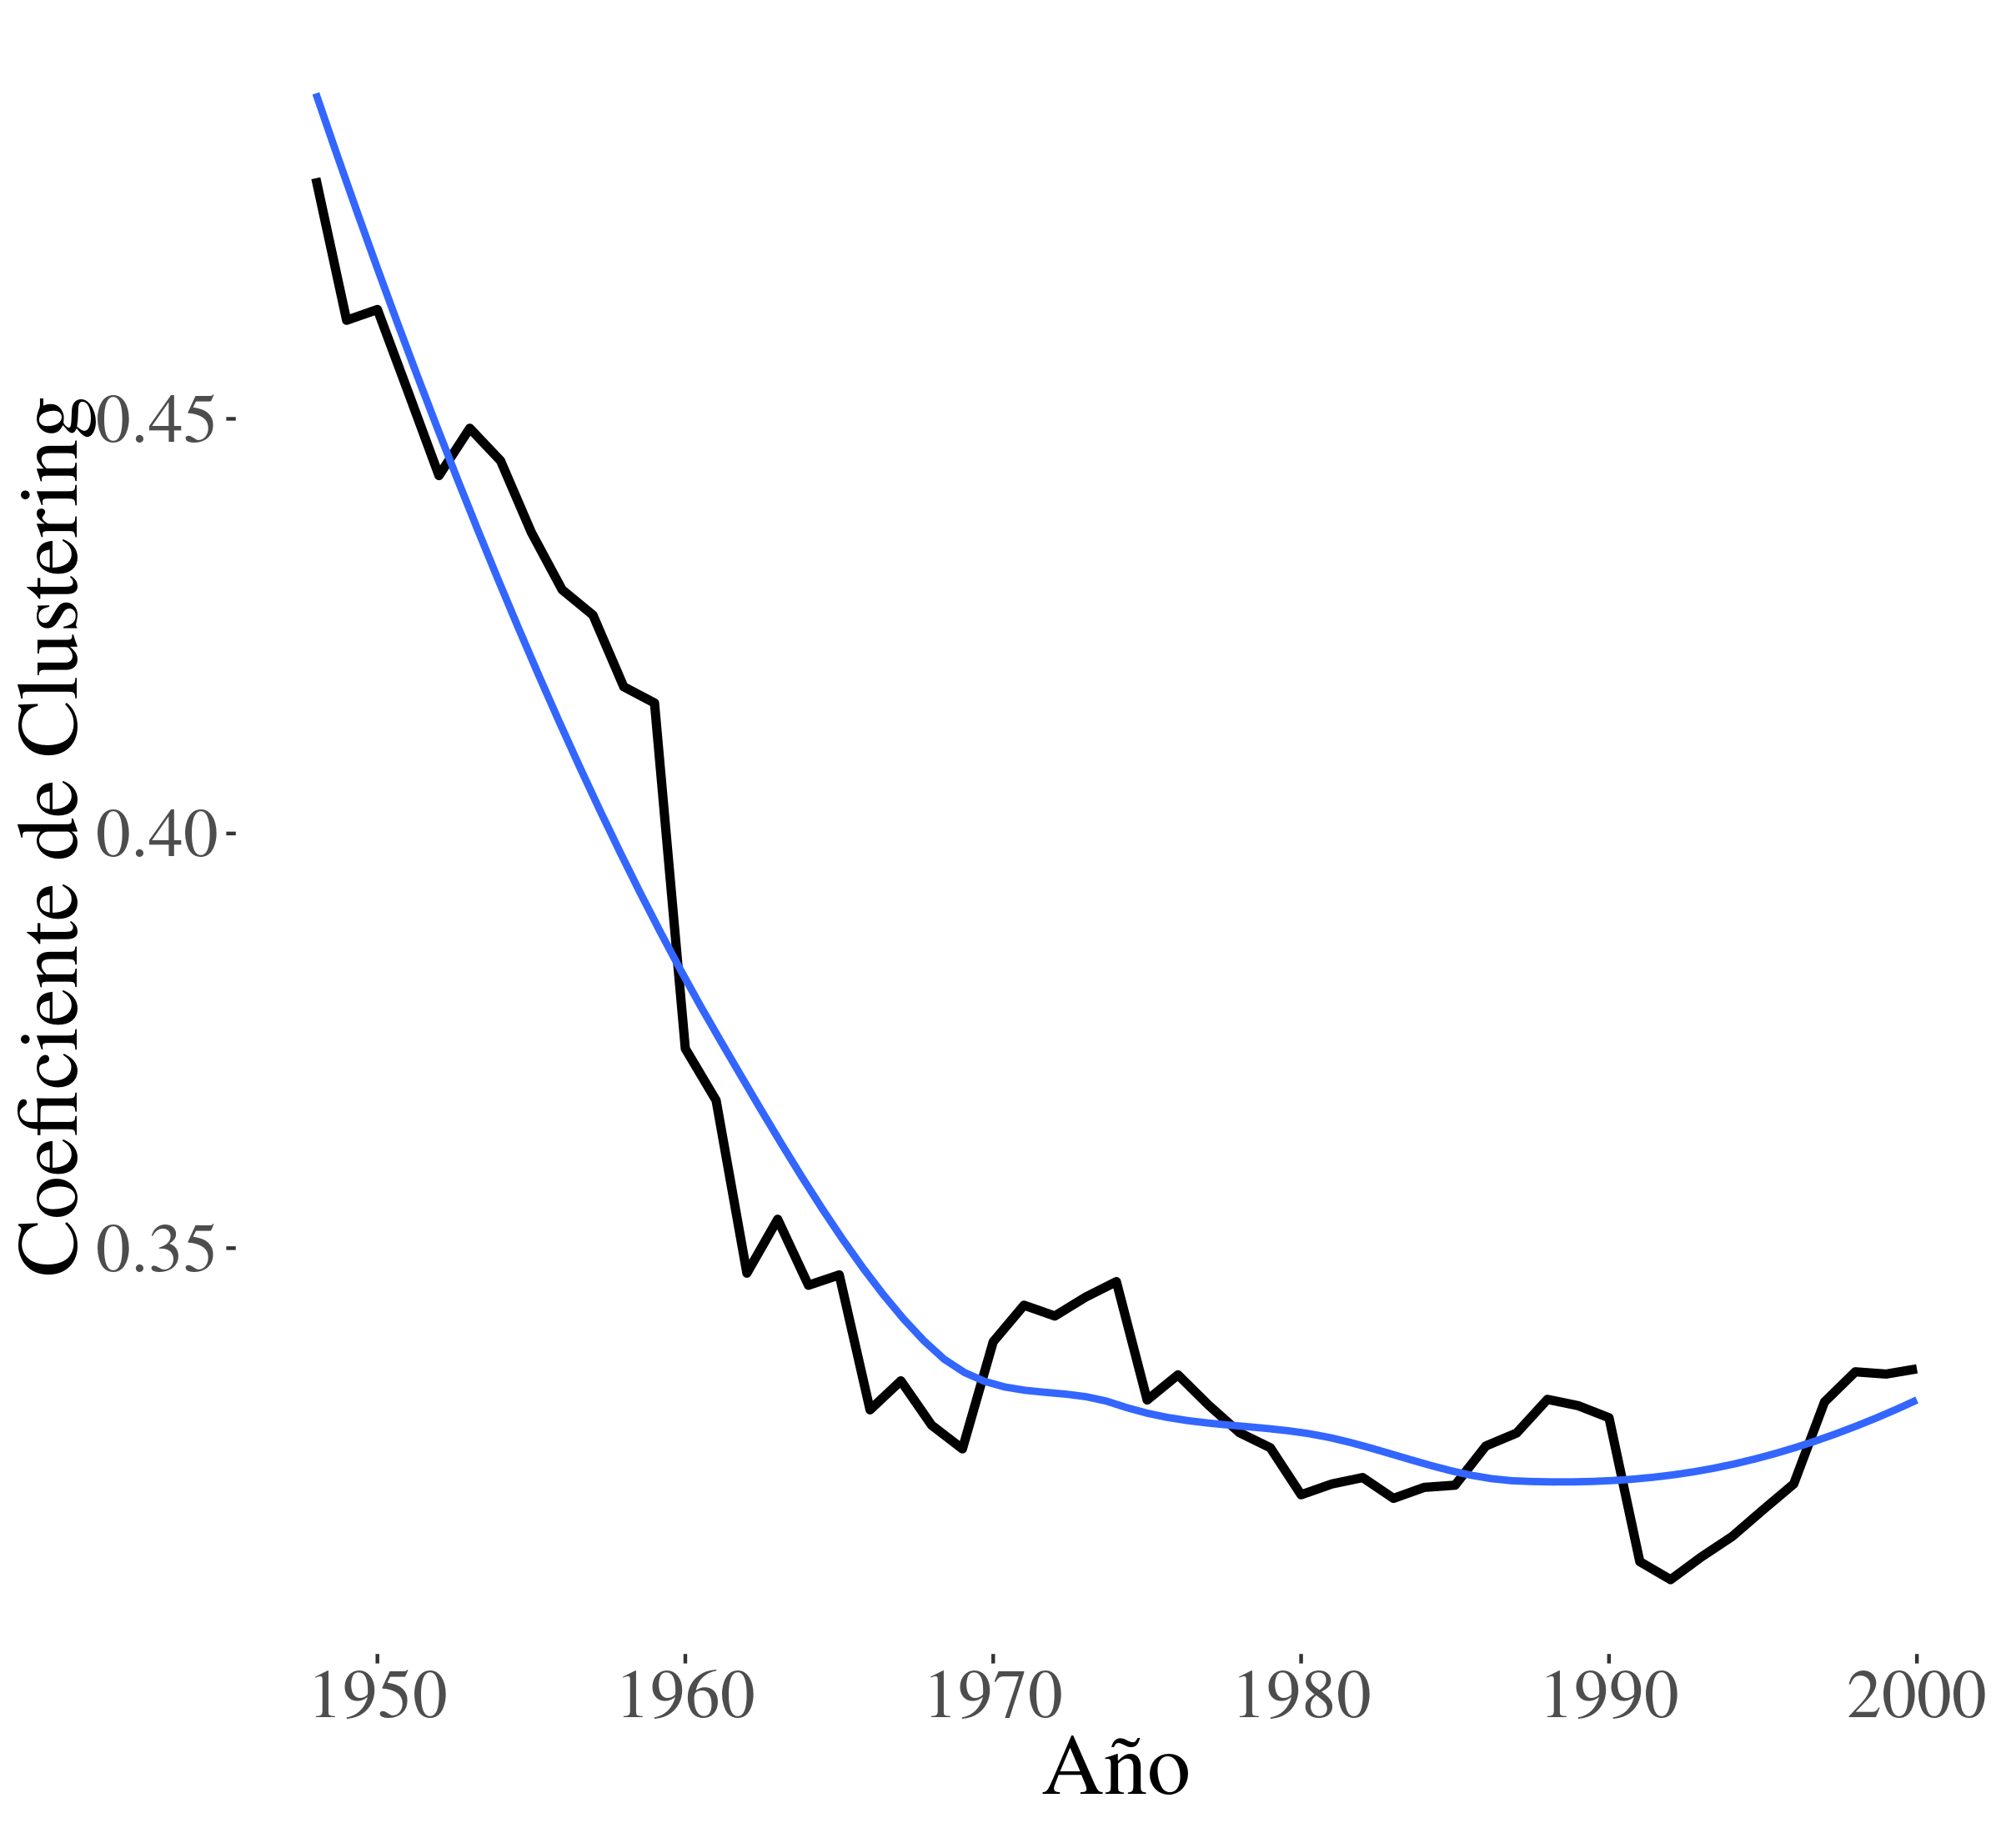
\includegraphics[width=.48\linewidth]{1950_2000_coef_clustering_x_yr}}
	\subfigure{\label{fig:metricas_LP-b}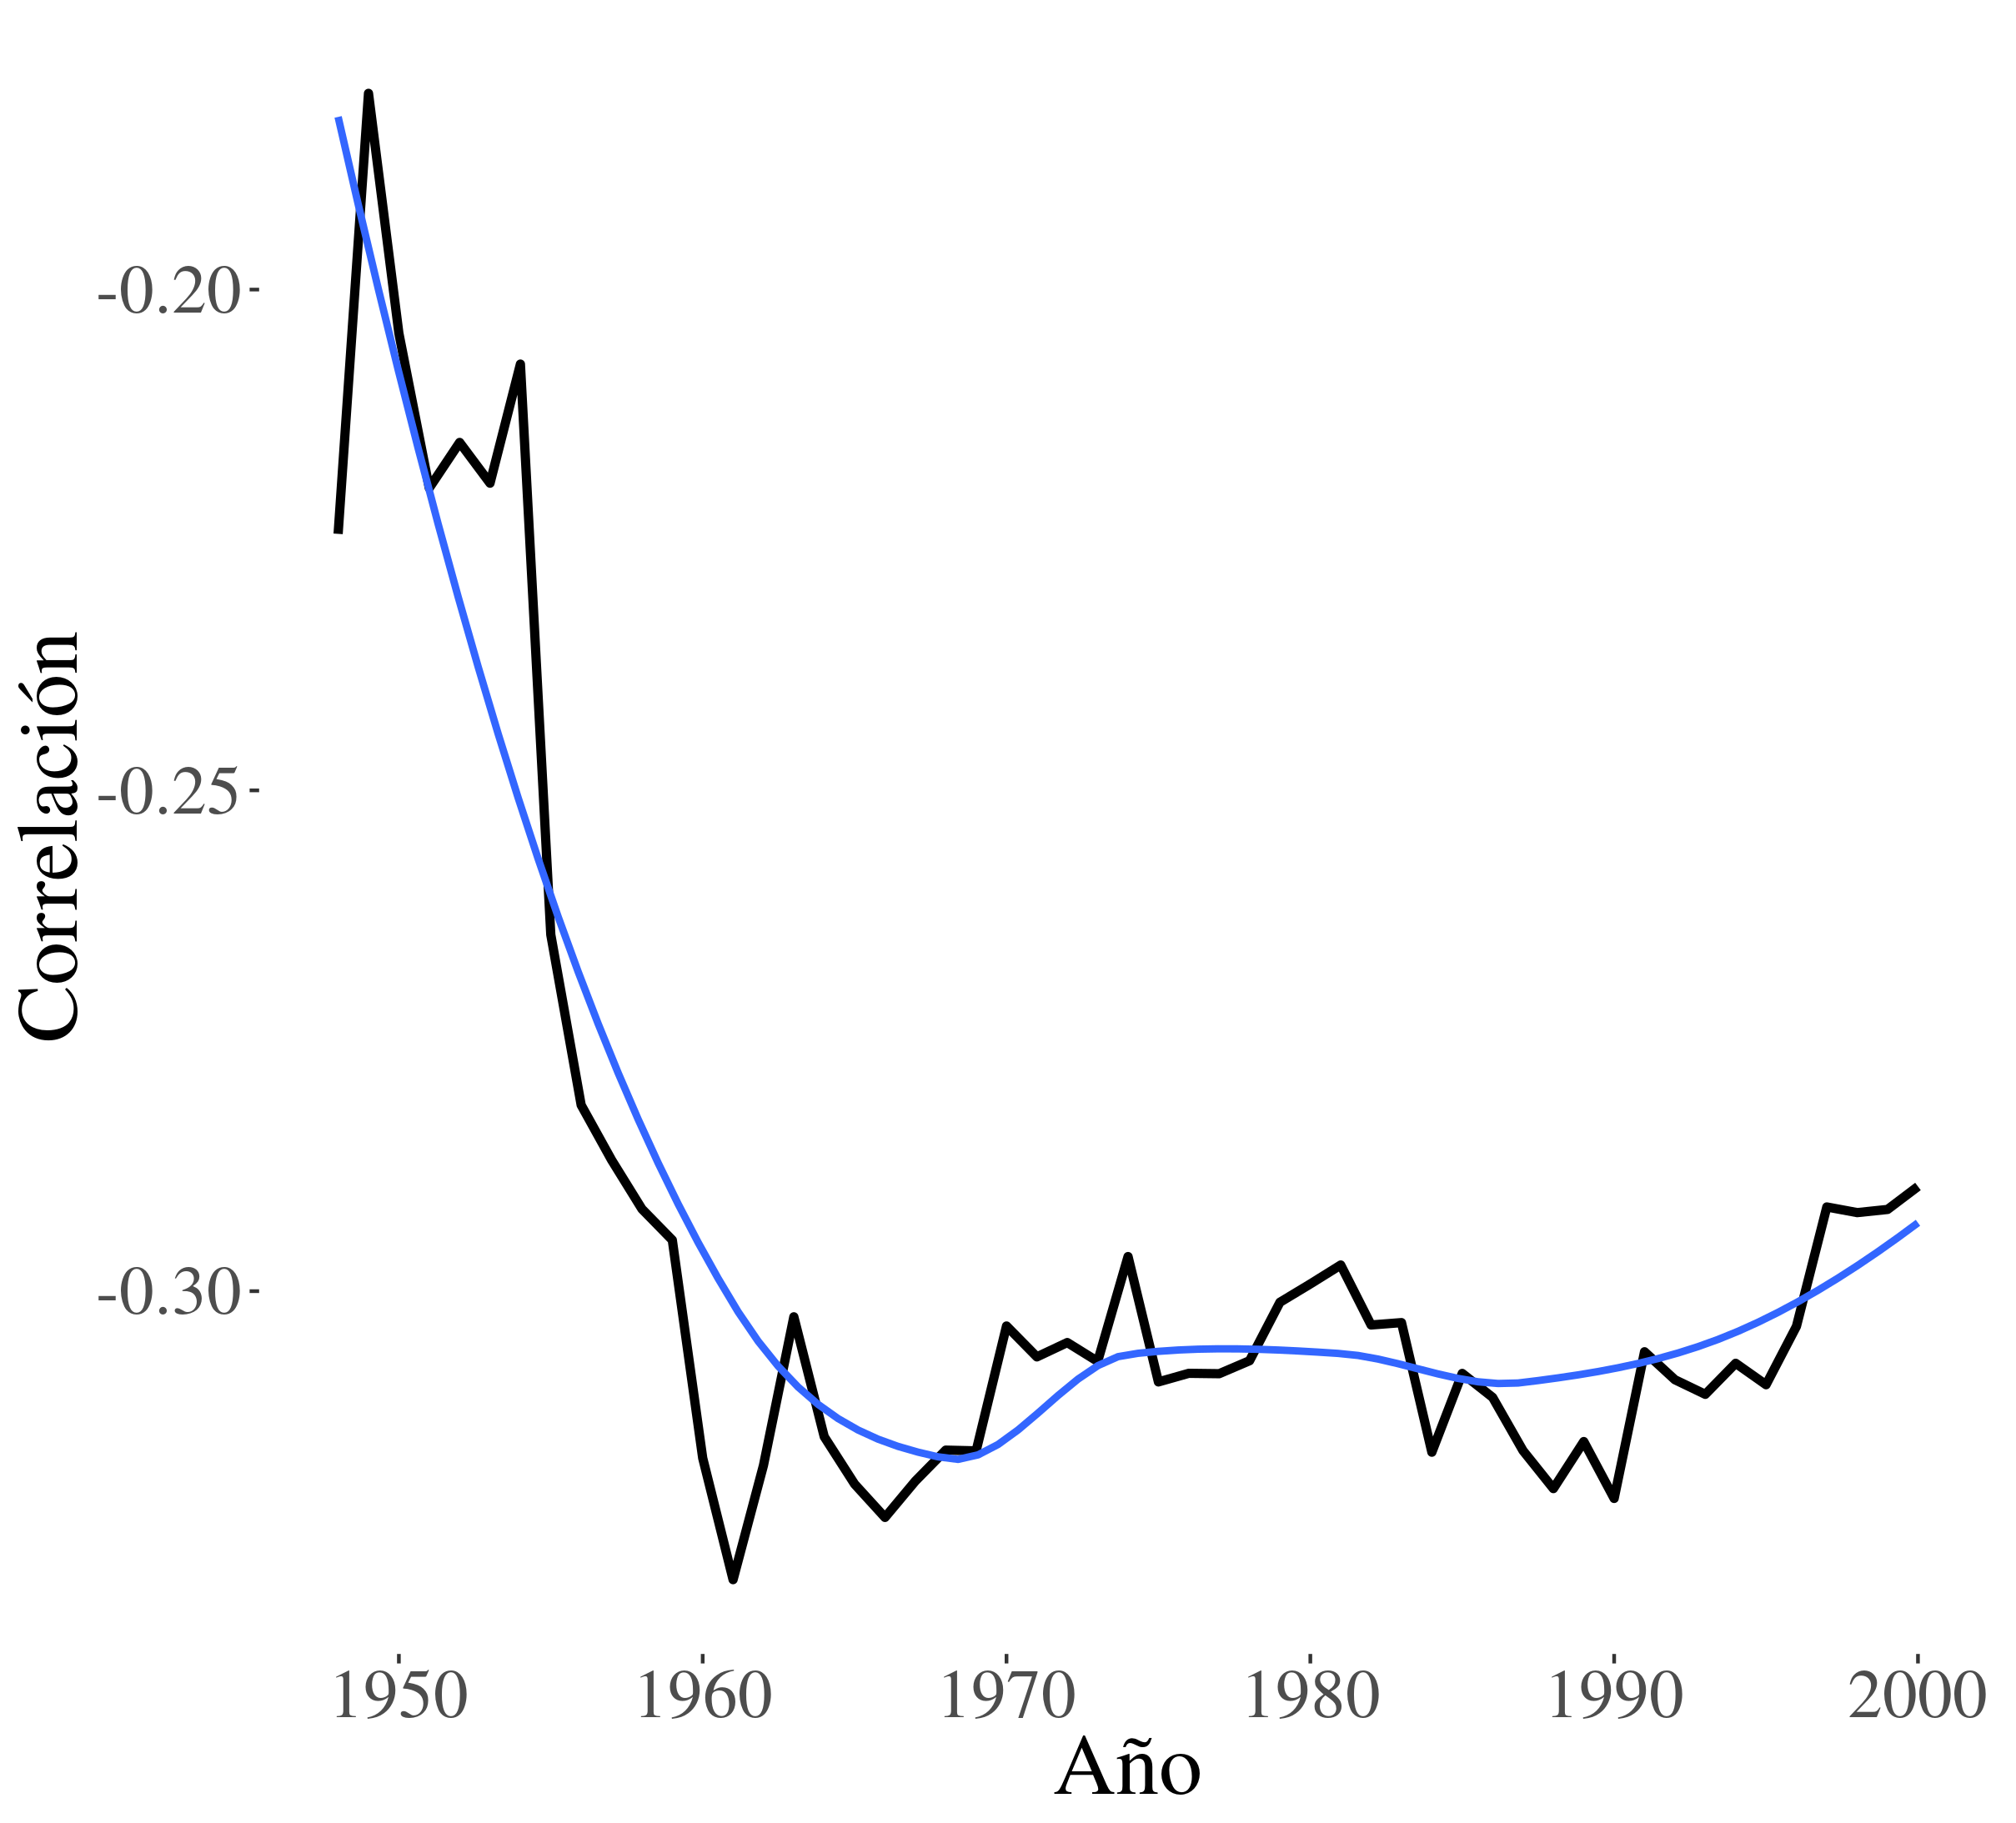
\includegraphics[width=.48\linewidth]{1950_2000_correlacion_x_yr}}
	\caption*{\scriptsize Evolución de la estructura de la red. Importaciones. Umbral 1\%. 1948-2000}
	\label{fig:metricas_LP}
\end{figure}

\small
\begin{itemize}[label=\faRebel]
	\item En la segunda mitad del S XX se observa una tendencia a la \textit{clusterización } o regionalización de las relaciones comerciales.
	\item La caída de la correlación de grado indica un aumento de las relaciones entre países \textit{centrales} y \textit{periféricos}
\end{itemize}



\end{frame}

\begin{frame}
	\begin{figure}
		\centering		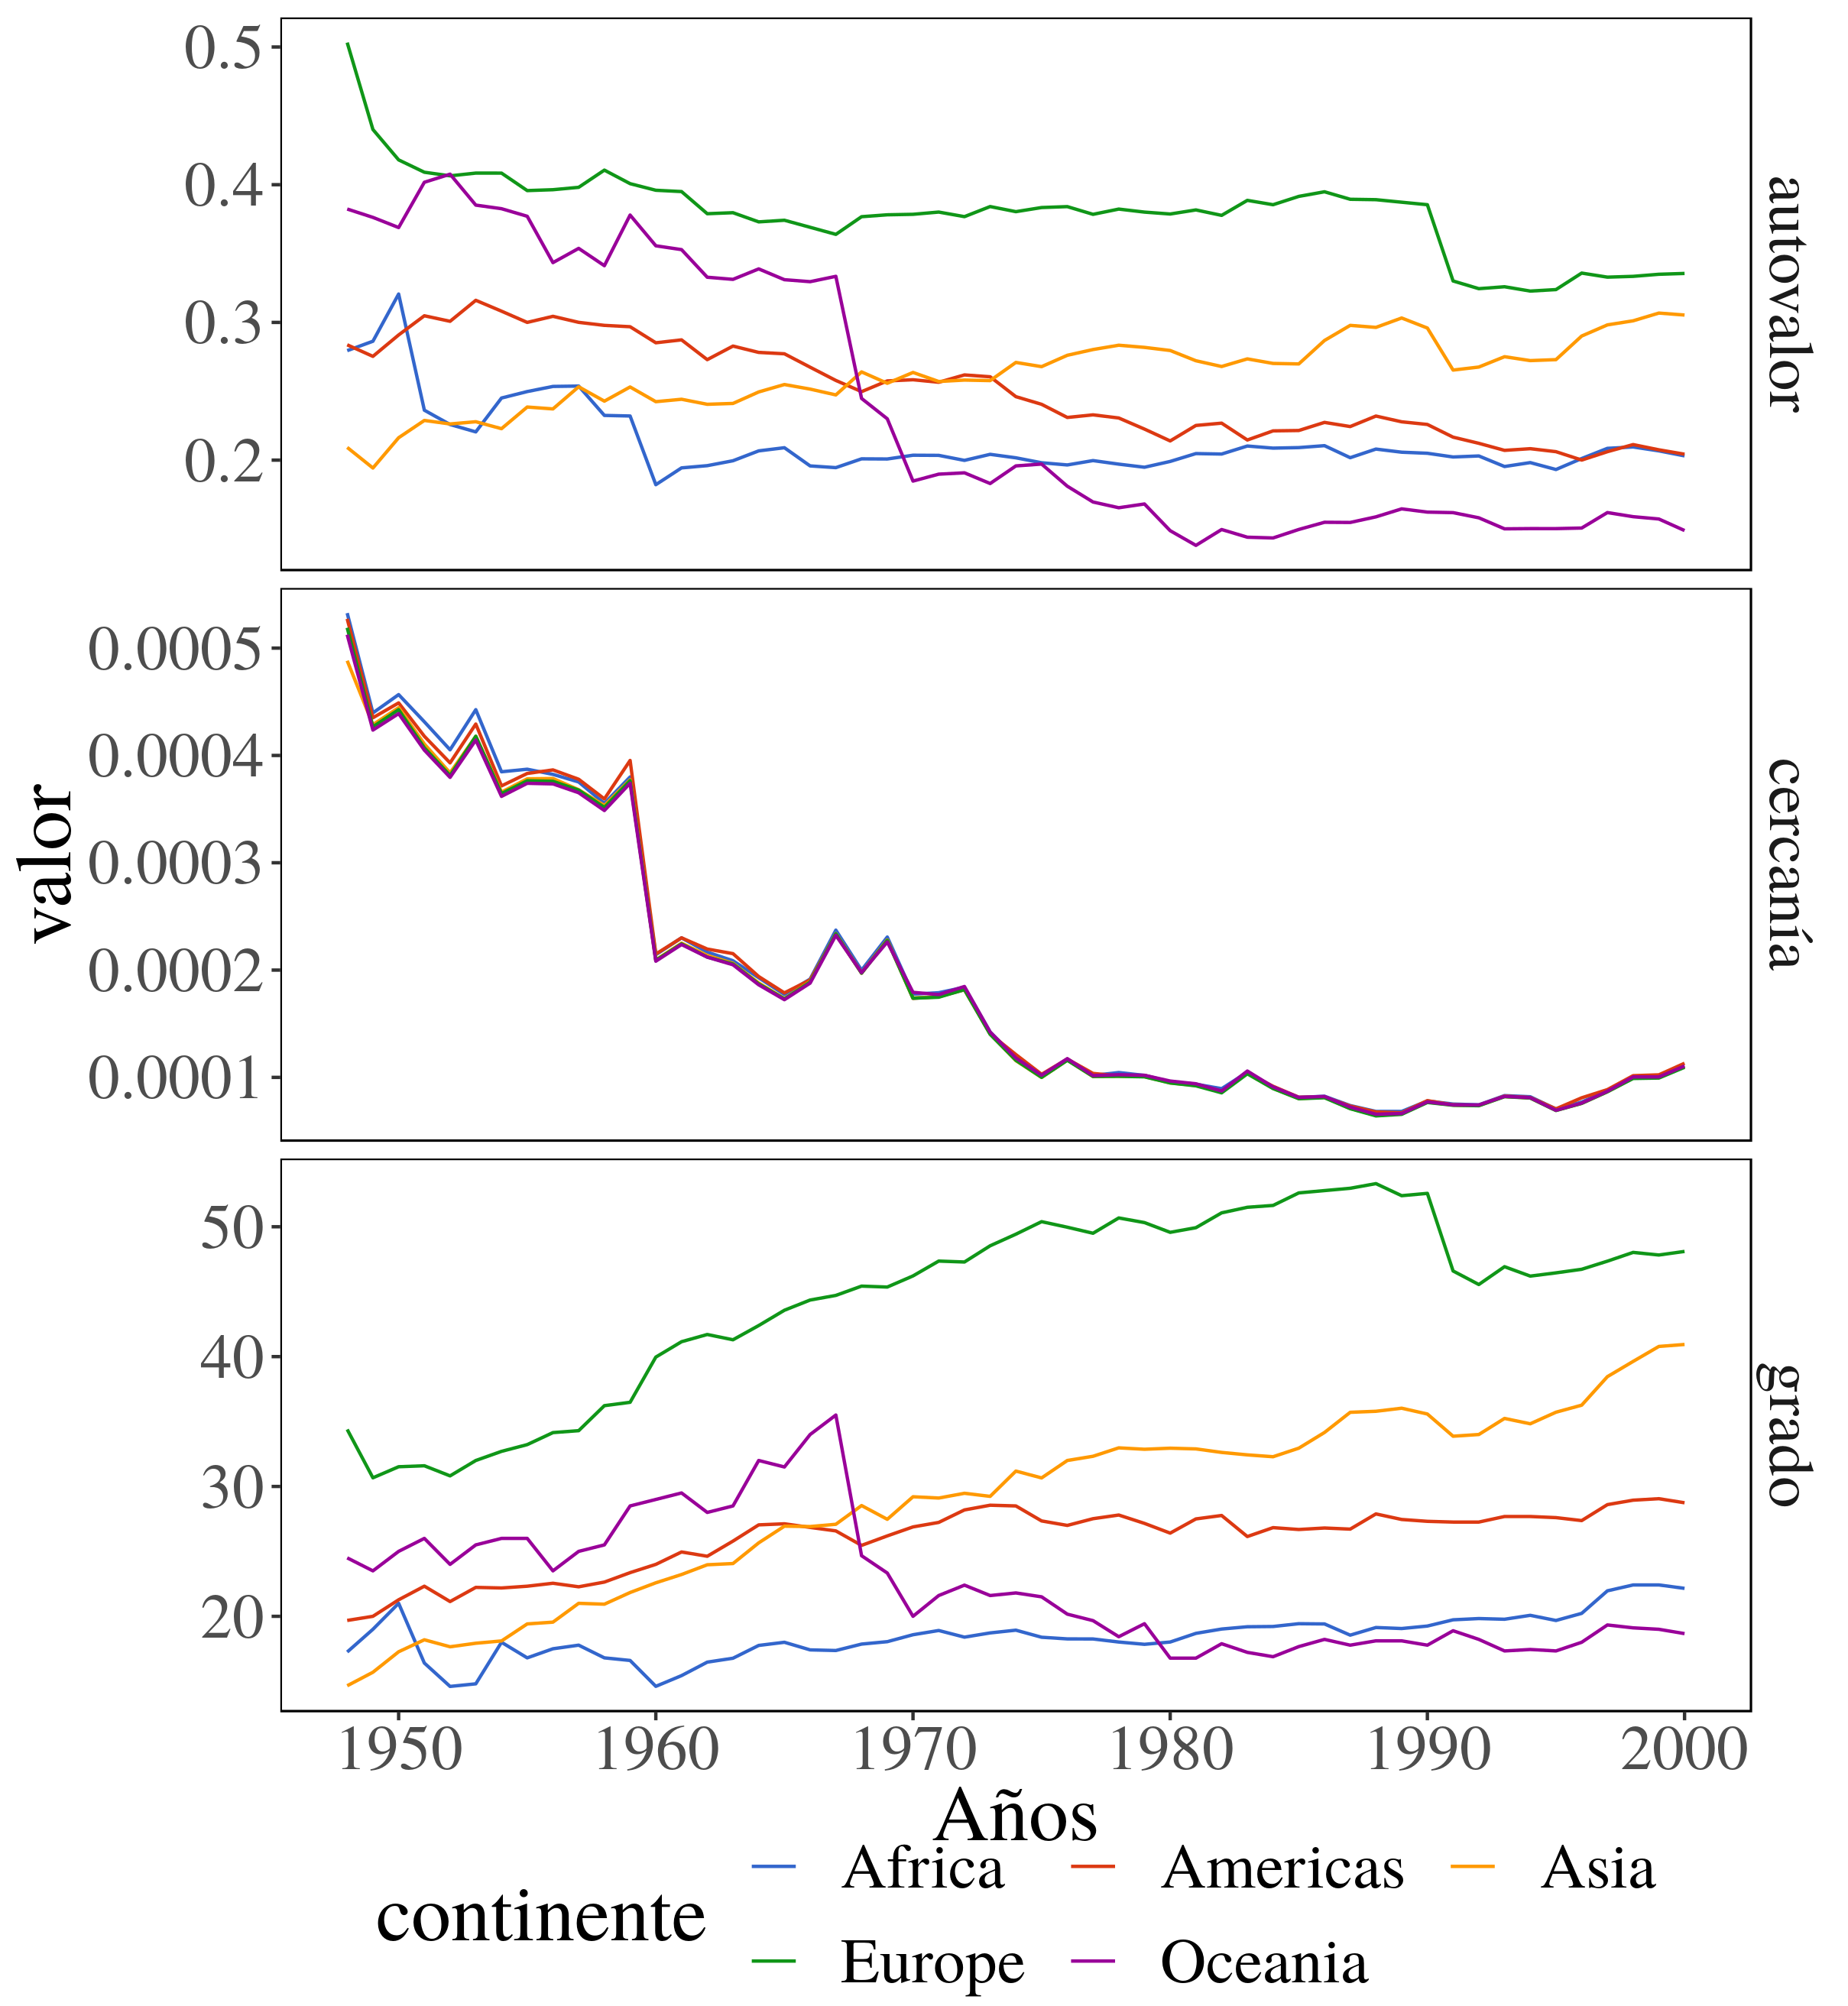
\includegraphics[width=0.75\linewidth]{1950_2000_continent_all}
		\caption{Evolución de la centralidad promedio por contiente. Impo. Umbral 1\%}
		\label{fig:centralidad_LP}
	\end{figure}
	
\end{frame}

\subsection{Value Chains}
\begin{frame}
\begin{figure}
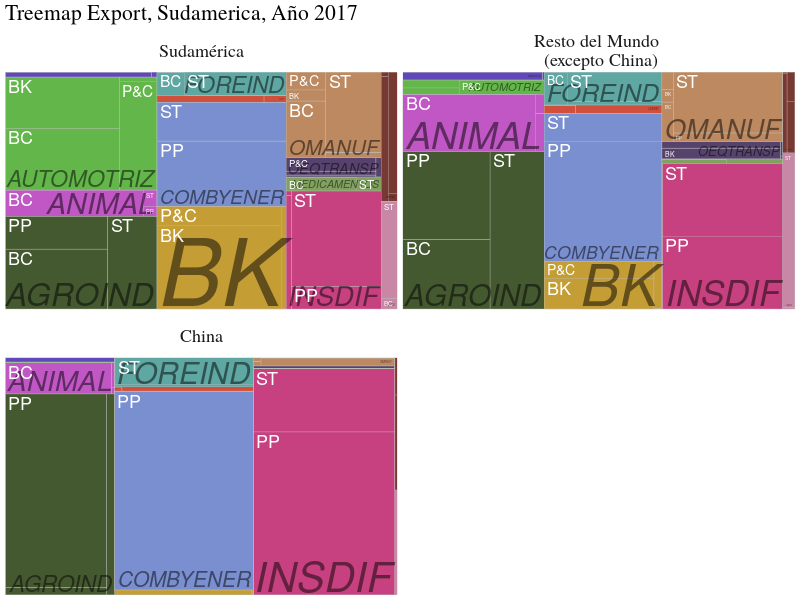
\includegraphics[scale=0.35]{uses_treemap}
\end{figure}

\small{Más resultados en: \textbf{\url{https://treemaps.shinyapps.io/LDA_worldtrade/}}}
\end{frame}



\subsection{Latent Dirichlet Allocation}
\begin{frame}
\begin{columns}[c] 

\column{.45\textwidth} % Right column and width
\small{Example of component}
\begin{figure}
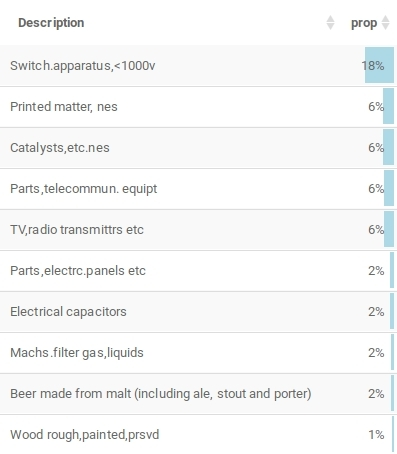
\includegraphics[scale=0.3]{LDA_comp}
\end{figure}

\column{.7\textwidth} % Left column and width

\small{This components can then be used for analyze the trend in world trade} \par
\begin{flushleft}
\begin{figure}
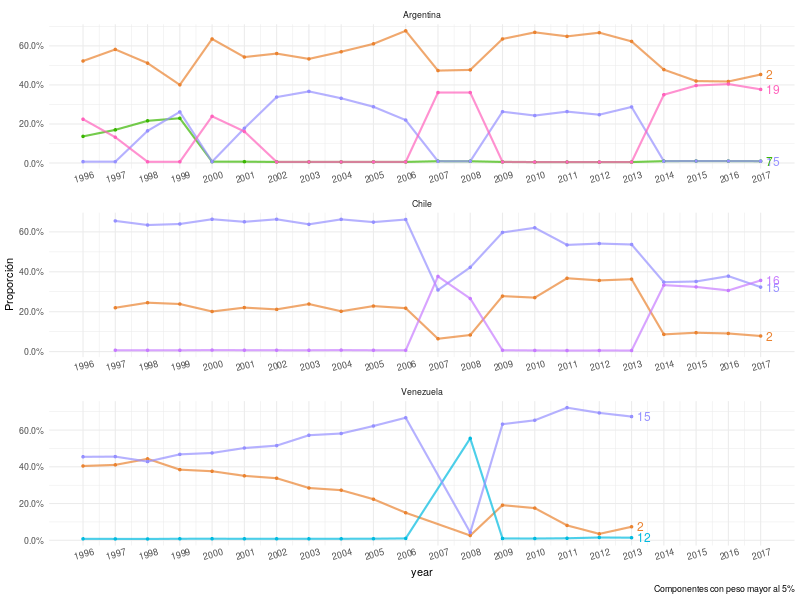
\includegraphics[scale=0.25]{LDA_res}
\end{figure}
\end{flushleft}

\end{columns} 
\medskip
\small{More results in: \textbf{\url{https://treemaps.shinyapps.io/shiny_LDA/}}}
\end{frame}

\end{document}